
\chapter{Results and Discussion}

\label{Chapter5} % For referencing the chapter elsewhere, use \ref{Chapter1} 

\section{Results}

To test the AI's performance, we set up the following experiment. First, the subject was given time to familiarize and acclimate themselves to the controls and dynamics of the game. Afterwards, the subject played five 20 second long matches against a computer opponent that follows a set defensive behavior pattern. A random set of matches from this pool was selected to be the demonstration sessions, while the rest were grouped into a set of holdout sessions. We then used the data from the demonstration session to create three kinds of agents. One of the agents used our novel search technique. We refer to this agent as Search AI. The other agents implemented an simple N-gram AI and the adaptive Ghost AI and served as a point of comparison. An N-gram AI is essentially a vanilla GhostAI that is not aware of the current game state. We then recorded several sessions where each of these agents was pitted against the same computer opponent that the subject faced.

We performed several kinds of experiments. In one, one session was selected to be the demonstration session. In another, the agents half of the available sessions were selected as the demonstration session. In the last one, the opponent used for the demonstrations and during the demonstration was a human opponent. Half of the available sessions were selected as the demonstration session and the human opponent was kept consistent through all of sessions.

The recorded sessions were evaluated along three criteria: Similarity, Effectiveness, and Qualitative Analysis. 

The data on the tables are interpreted as follows. The mean refers to the mean of all of the similarity scores. The Avg. Standard Deviation refers to the average of the standard deviation within each player's mimicking agent. So Player A's N-gram AI may have a similarity standard deviation of 1, Player B's may have a similarity standard deviation of 2, so the Avg Standard Deviation of the N-gram AI would be 1.5

\subsection{Similarity}

To measure similarity, we used a metric based on the work by \cite{simil}. The metric works as follows. Given event sequences $A$ and $B$, let $H_A$ and $H_B$ represent the underlying histogram of all $n$-Grams where $1 \le n \le 3$. Then let $S_A$ and $S_B$ be the number of unique substrings in $H_A$ and $H_B$ respectively, and let $f(s|H)$ be the number of times substring $s$ appears in histogram $H$. The similarity metric is then defined as follows:

$$PlayerSim(A,B) = \sum_{s \in S_A \cup S_B} \frac{|f(s|H_A) - f(s|H_B)|}{f(s|H_A) + f(s|H_B)}$$

We recorded the similarity between and each AI's test sessions and the holdout sessions and report them below. We also include the similarity between the demonstration and holdout sessions as a point of comparison. 

%\begin{table}[h]
%	\centering
%	\caption{ Similarity Measurements }
%	\begin{tabular}	{| c | c | c | c | c |}
%		\hline
%		 & Holdout Session & N-gram & GhostAI & Search AI \\
%		\hline
%		Mean &
%		0.447 & 0.224 & 0.265 & 0.248\\
%		\hline
%		Standard Deviation & 
%		0.078 & 0.047 & 0.036 & 0.034\\
%		\hline
%	\end{tabular}
%	\label{Similarity}
%\end{table}

\begin{table}[h]
	\centering
	\caption{ Similarity Measurements: One Demonstration }
	\begin{tabular}	{| c | c | c | c | c |}
		\hline
		& Holdout Session & N-gram & GhostAI & Search AI \\
		\hline
		Mean &
		0.447&
		0.191&
		0.242&
		0.237\\
		\hline
		Avg. Standard Deviation & 
		0.078 &
		0.057 &
		0.033 &
		0.040 \\
		\hline
	\end{tabular}
	\label{Similarity}
\end{table}

\begin{table}[h]
	\centering
	\caption{ Similarity Measurements: Half of the Demonstrations }
	\begin{tabular}	{| c | c | c | c | c |}
		\hline
		& Holdout Session & N-gram & GhostAI & Search AI \\
		\hline
		Mean &
		0.436&
		0.210&
		0.221&
		0.181\\
		\hline
		Avg. Standard Deviation & 
		0.085&
		0.047&
		0.035&
		0.028\\
		\hline
	\end{tabular}
	\label{Similarity}
\end{table}

\begin{table}[h]
	\centering
	\caption{ Similarity Measurements: Human Play }
	\begin{tabular}	{| c | c | c | c | c |}
		\hline
		& Holdout Session & N-gram & GhostAI & Search AI \\
		\hline
		Mean &
		0.301 &
		0.136 &
		0.168 &
		0.165\\
		\hline
		Avg. Standard Deviation & 
		0.054 &
		0.033 &
		0.048 &
		0.017\\
		\hline
	\end{tabular}
	\label{Similarity}
\end{table}

From a similarity point of view the algorithm does decently. When given a single sessions worth of demonstration, the Search AI compares favorably to GhostAI and surpasses the N-gram AI. However, once more data is added to the demonstration data set, Search AI's performance begins to fall off while N-gram improves and overtakes it. This is likely because of the increased number of demonstrated actions increases the number of state successors when taking $\delta$-transitions, slowing down the search. The Search AI's low standard deviation is expected, as its planning-based behavior should have less of the chaotic randomness shown by the other AI.

Taking a closer look at the data points where the AI's have more demonstrations, the instances where Search AI did dramatically better than the N-gram AI and the instances where it did dramatically worse were split fairly evenly. In the instances where we saw worse performance, the Search AI would repeatedly attack in place until the predictor could update and have create a more feasible plan. This shows the Search AI may be able to achieve high similarity with larger data sets if it can learn to overcome these planning local minima. 

Lastly, the similarity measurements for human-play are mostly in-line with the similarity when pit against an computer opponent. Despite having more demonstration data, the Search AI is able to keep pace with the GhostAI and outperform the N-gram AI. This likely happens because the human-opponent rarely lets the Search AI form poor local minima plans, as they will hit and interrupt it before it can get stuck for an extended period.

\subsection{Effectiveness}
To measure Effectiveness, we compared the number of hits that were landed in the training session to the average number of hits recorded for each other category. We also compared the average number of actions that needed to be performed to land a hit. We rec

\begin{table}[h]
	\centering
	\caption{Hits Landed Per Session: : One Demonstration }
	\begin{tabular}	{| c | c | c | c | c | }
		\hline
		& Original Player & N-gram & GhostAI & Search AI \\
		\hline
		Mean &
		6.75 & 2.6 & 2.35 & 4\\
		\hline
		Avg. Standard Deviation &
		1.55 & 1.162 & 0.683 & 1.368\\
		\hline
	\end{tabular}
	\label{Effectiveness1}
\end{table}


\begin{table}[h]
	\centering
	\caption{Actions required per Hit:  One Demonstration }
	\begin{tabular}	{| c | c | c | c | c | }
		\hline
		& Original Player & N-gram & GhostAI & Search AI \\
		\hline
		Mean &
		10.54 & 22.49 & 36.83 & 11.45\\
		\hline
		Avg. Standard Deviation &
		3.77 & 11.54 & 19.39 & 2.66\\
		\hline
	\end{tabular}
	\label{Effectiveness2}
\end{table}

From an effectiveness point of view, the search AI is definitely more effective compared to the other 2. Not only does it on average land more hits per session, it also uses fewer actions to achieve those hits. This makes sense because the Search AI tries to create plans that let it reach a goal state relatively efficiently, whereas N-gram and GhostAI are constantly performing actions. Its also good to see that the Search AI's requires roughly the same number of actions to land a hit as the original players. It shows that the AI is not just taking an optimal path to the goal, but is in some way matching the success-rate of the player it is emulating. 

One thing that is odd is that the Ghost AI seems to perform worse than the N-gram AI in this category. This is probably because the Ghost AI does not receive a penalty if an opponent blocks an attack, meaning that in one instance it could hit the opponent and then be tricked into thinking that action is always the best one to take to maximize reward.

\begin{table}[h]
	\centering
	\caption{Hits Landed Per Session:  Half of the Demonstrations }
	\begin{tabular}	{| c | c | c | c | c | }
		\hline
		& Original Player & N-gram & GhostAI & Search AI \\
		\hline
		Mean &
		6.75&
		3.15&
		2.4&
		2.7\\
		\hline
		Avg. Standard Deviation &
		1.546&
		2.041&
		1&
		1.186\\
		\hline
	\end{tabular}
	\label{Effectiveness1}
\end{table}
\begin{table}[h]
	\centering
	\caption{Actions required per Hit:  Half of the Demonstrations }
	\begin{tabular}	{| c | c | c | c | c | }
		\hline
		& Original Player & N-gram & GhostAI & Search AI \\
		\hline
		Mean &
		10.541&
		20.079&
		37.835&
		16.259\\
		\hline
		Avg. Standard Deviation &
		3.776&
		7.200&
		10.670&
		2.610\\
		\hline
	\end{tabular}
	\label{Effectiveness2}
\end{table}

When we increase the amount of demonstration data, the Search AI's performance worsens by a significant margin. This is likely due to the fact that we are able to expand less states in the limited amount of time given due to the increase number of $\delta$-transitions.

\begin{table}[h]
	\centering
	\caption{Hits Landed Per Session: : Human Player}
	\begin{tabular}	{| c | c | c | c | c | }
		\hline
		& Original Player & N-gram & GhostAI & Search AI \\
		\hline
		Mean &
		6.8&
		4.4&
		3.8&
		9.4\\
		\hline
		Avg. Standard Deviation &
		5.418&
		5.953&
		2.482&
		4.224\\
		\hline
	\end{tabular}
	\label{Effectiveness1}
\end{table}


\begin{table}[h]
	\centering
	\caption{Actions required per Hit: Human Player}
	\begin{tabular}	{| c | c | c | c | c | }
		\hline
		& Original Player & N-gram & GhostAI & Search AI \\
		\hline
		Mean &
		9.588&
		17.727&
		12.684&
		5.809\\
		\hline
		Avg. Standard Deviation &
		0.540 &
		2.197885296&
		6.929140424&
		0.384684368\\
		\hline
	\end{tabular}
	\label{Effectiveness2}
\end{table}

Against a human player it's surprising to see that the Search AI is actually more effective than even the original player. This is probably because the Search AI is potentially able to stitch together the original players actions to create more effective strategies that the original player might not even have considered. Additionally, the Search AI is able to pick the best parts of all of the mimicked players demonstrations and use them to greater effect against the opponent. Lastly, the human-player takes offensive actions unlike the defensive AI, which make them more vulnerable to attacks in general. 

The scores for the N-gram and GhostAI are expectedly low. This is because neither the N-gram or GhostAI have the proper means for taking actions after being hit. The N-gram AI may try to take actions that are no longer available to it while it is knocked down, and though the GhostAI has some awareness of game context, if the world state is not the same as something encountered in the demonstration it is forced to pick from a uniform random distribution. 

\subsection{Qualitative Analysis}
For our qualitative analysis we also visually inspected heatmaps of the demonstrations like follows. We also analyzed the video footage of the different AI's

\begin{figure}[h]
	\centering
	\begin{subfigure}[h]{0.4\textwidth}
		\centering
		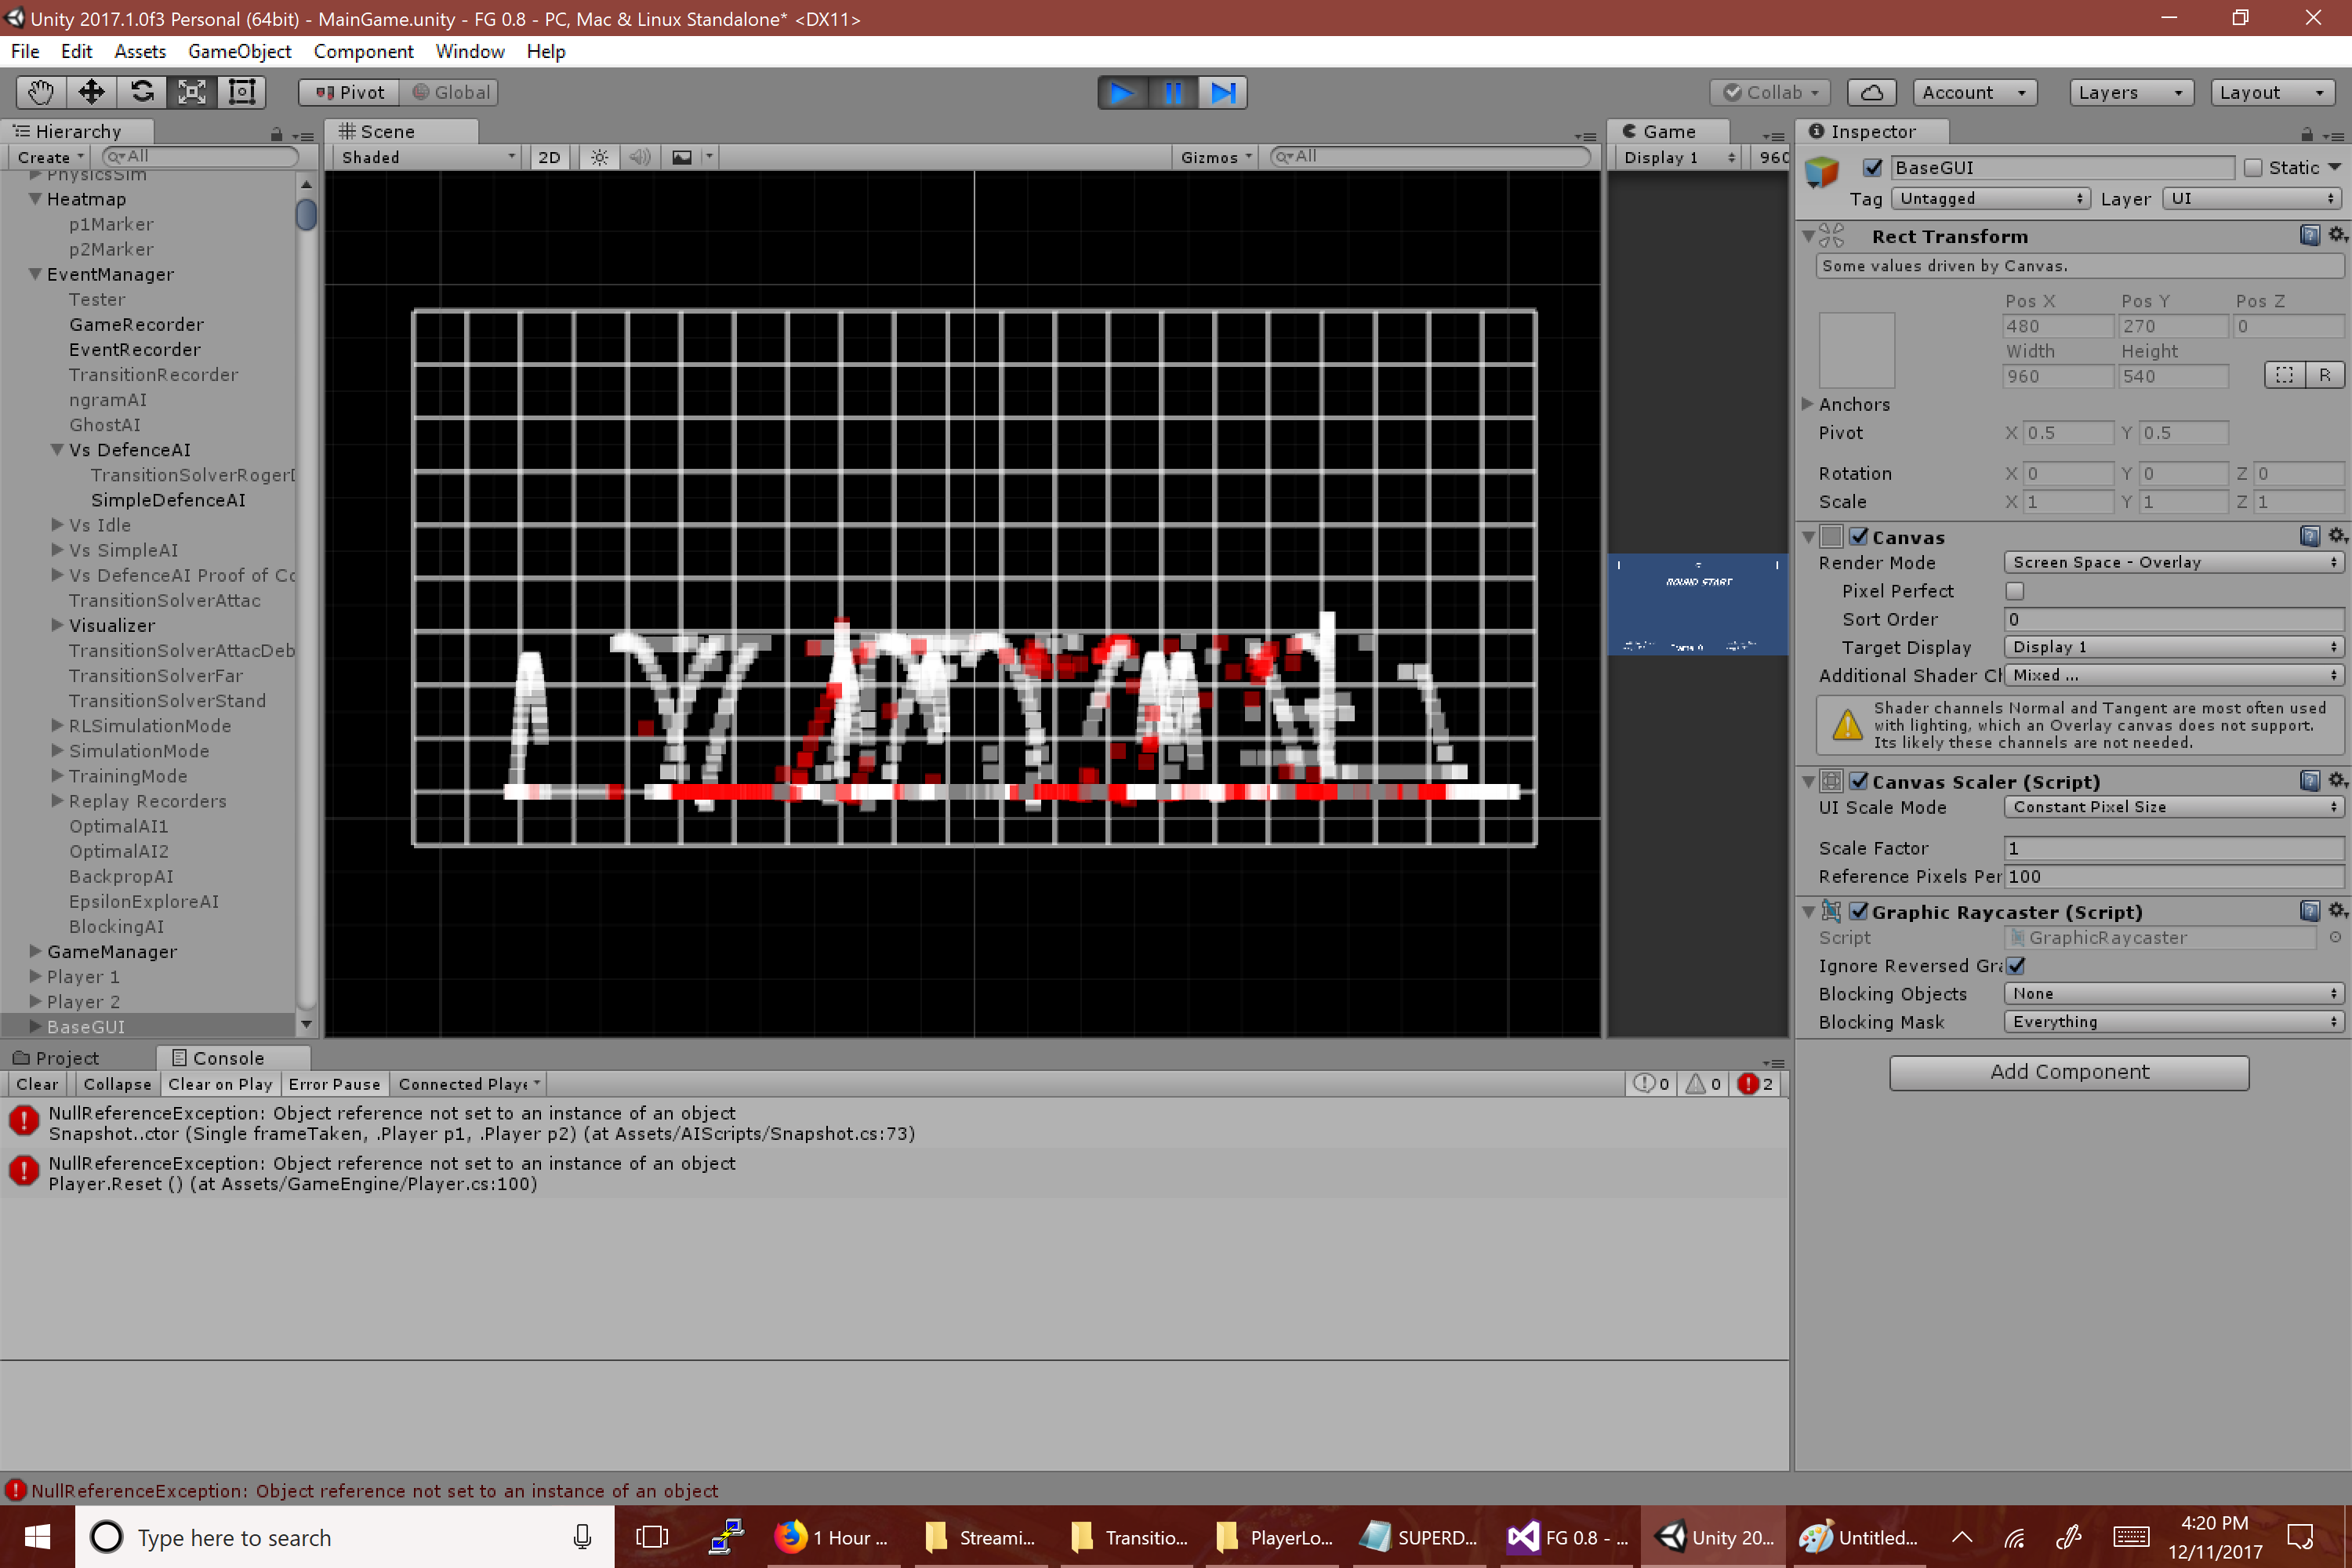
\includegraphics[width=\textwidth]{Figures/HeatmapOrig.png}
		\caption{Original Player Heatmap}
		\label{}
	\end{subfigure}
	\begin{subfigure}[h]{0.4\textwidth}
		\centering
		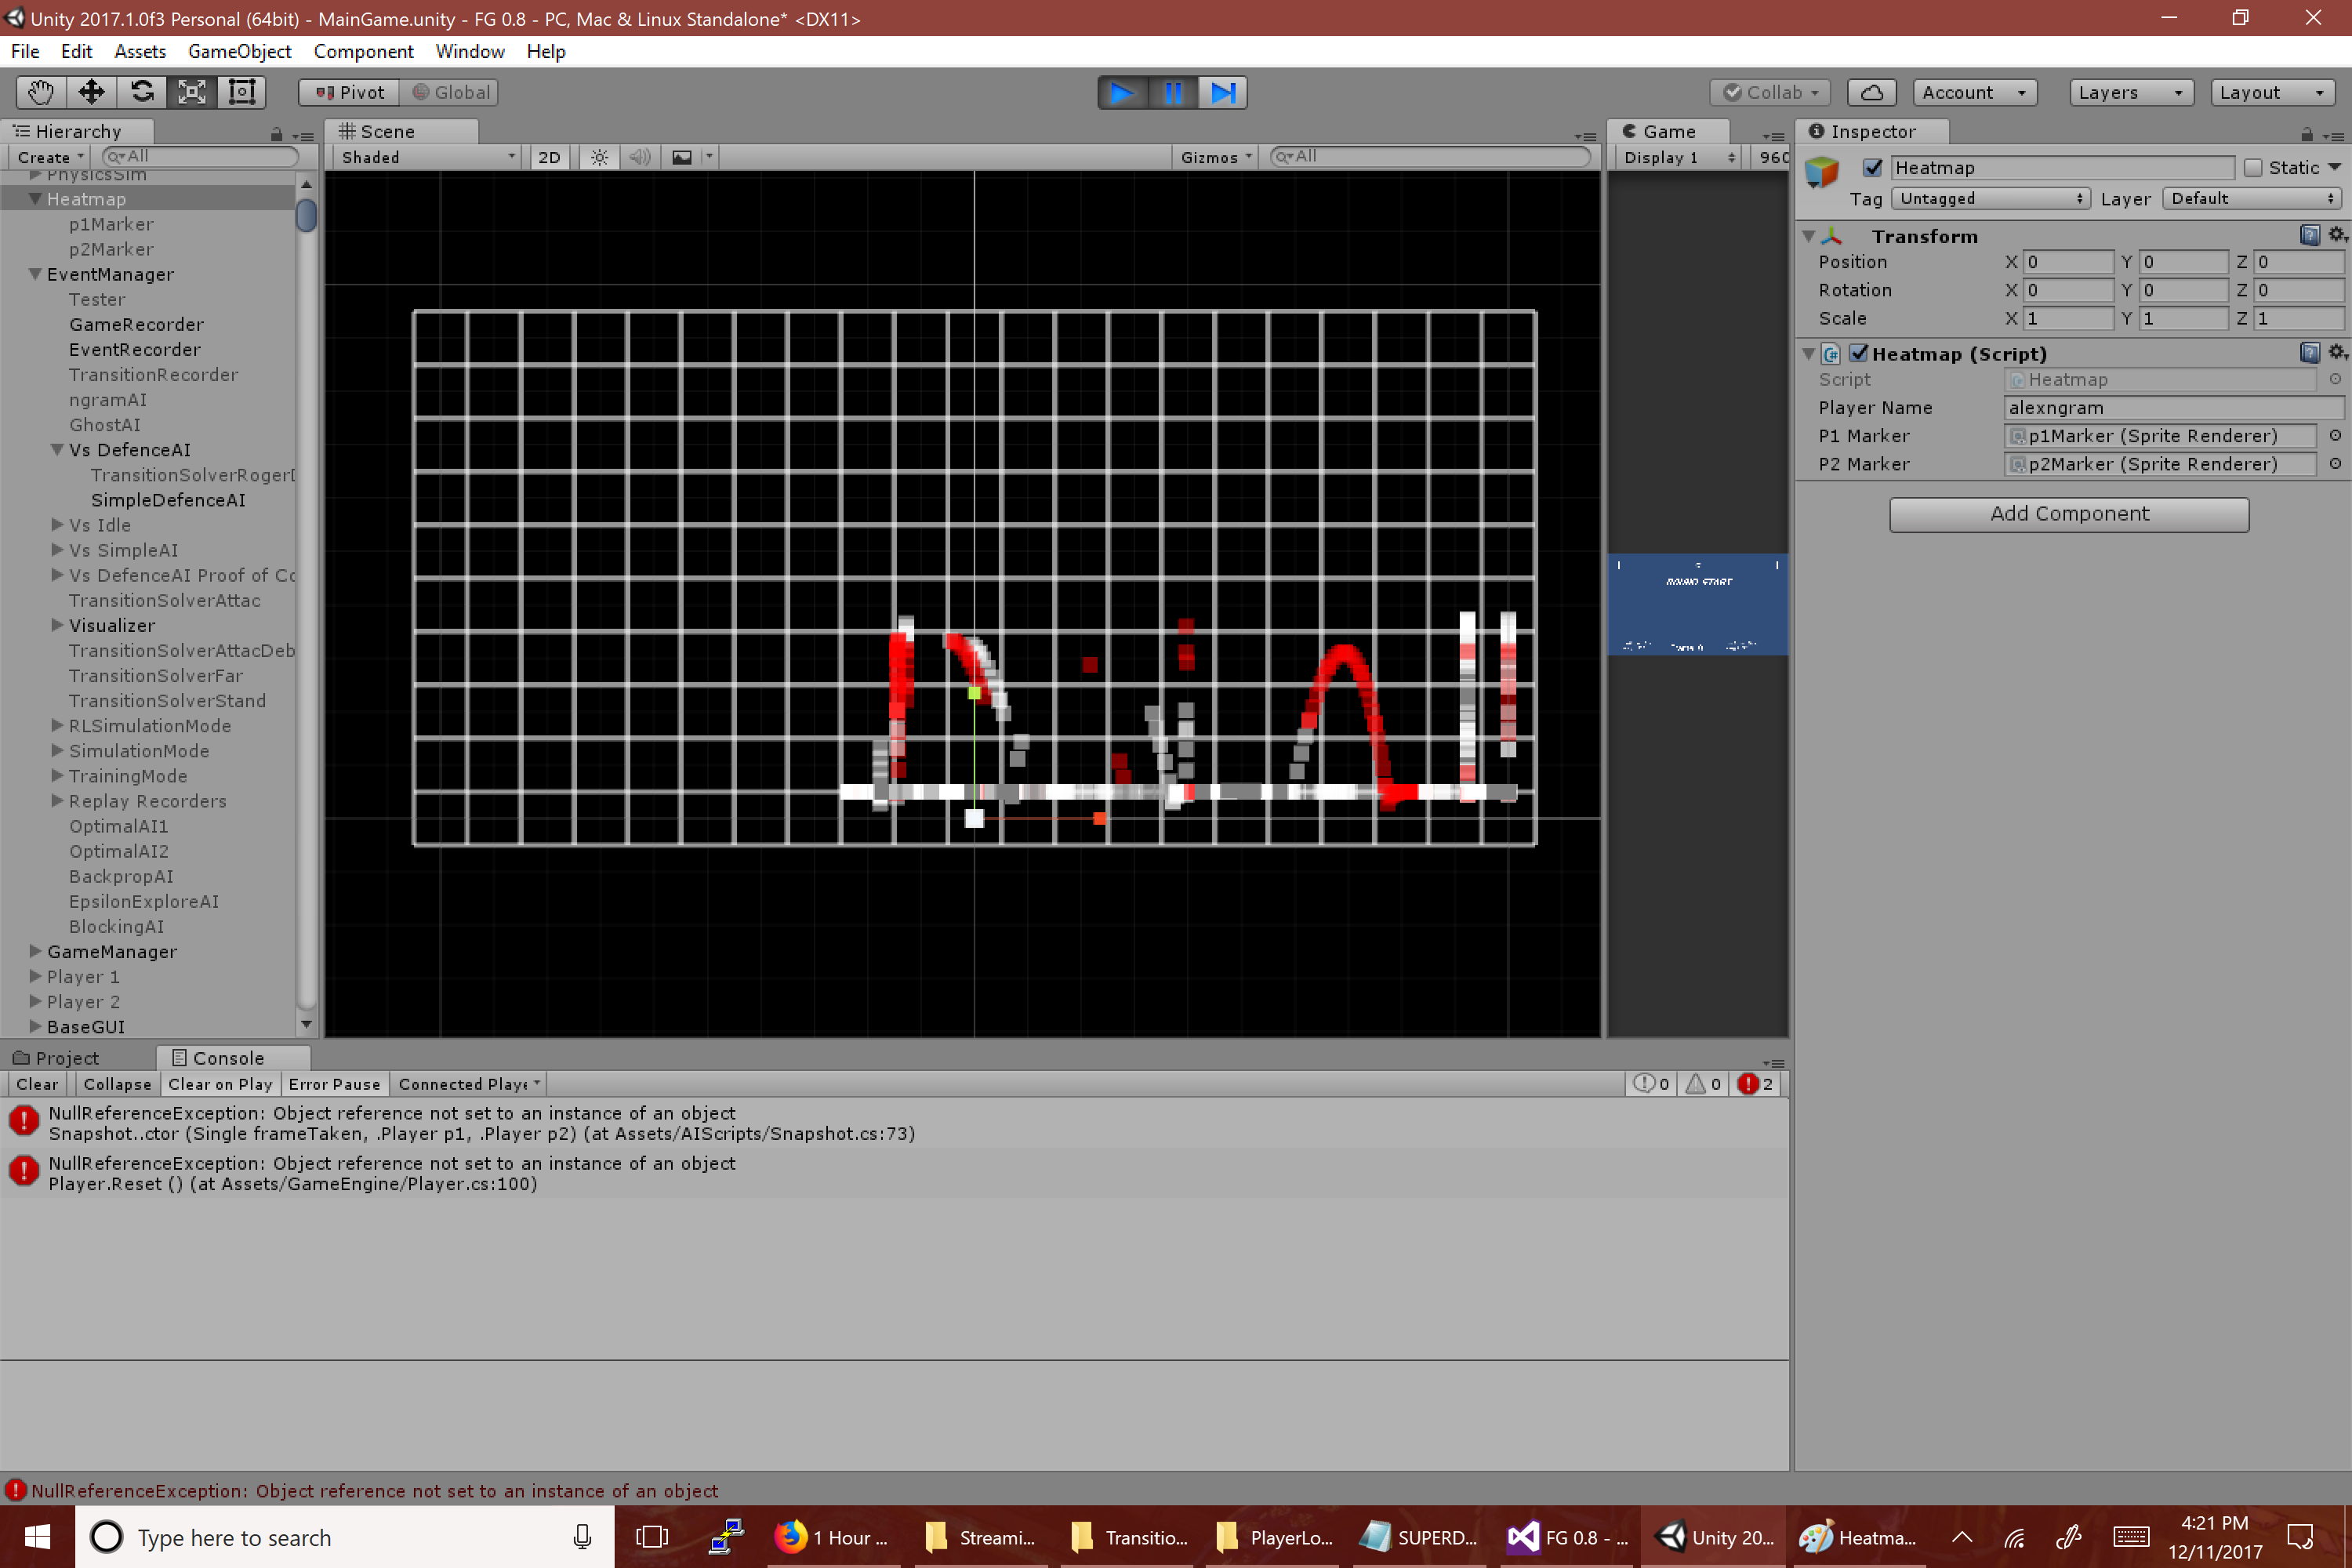
\includegraphics[width=\textwidth]{Figures/HeatmapNgram.png}
		\caption{N-gram AI Heatmap}
		\label{}
	\end{subfigure}
	\begin{subfigure}[h]{0.4\textwidth}
		\centering
		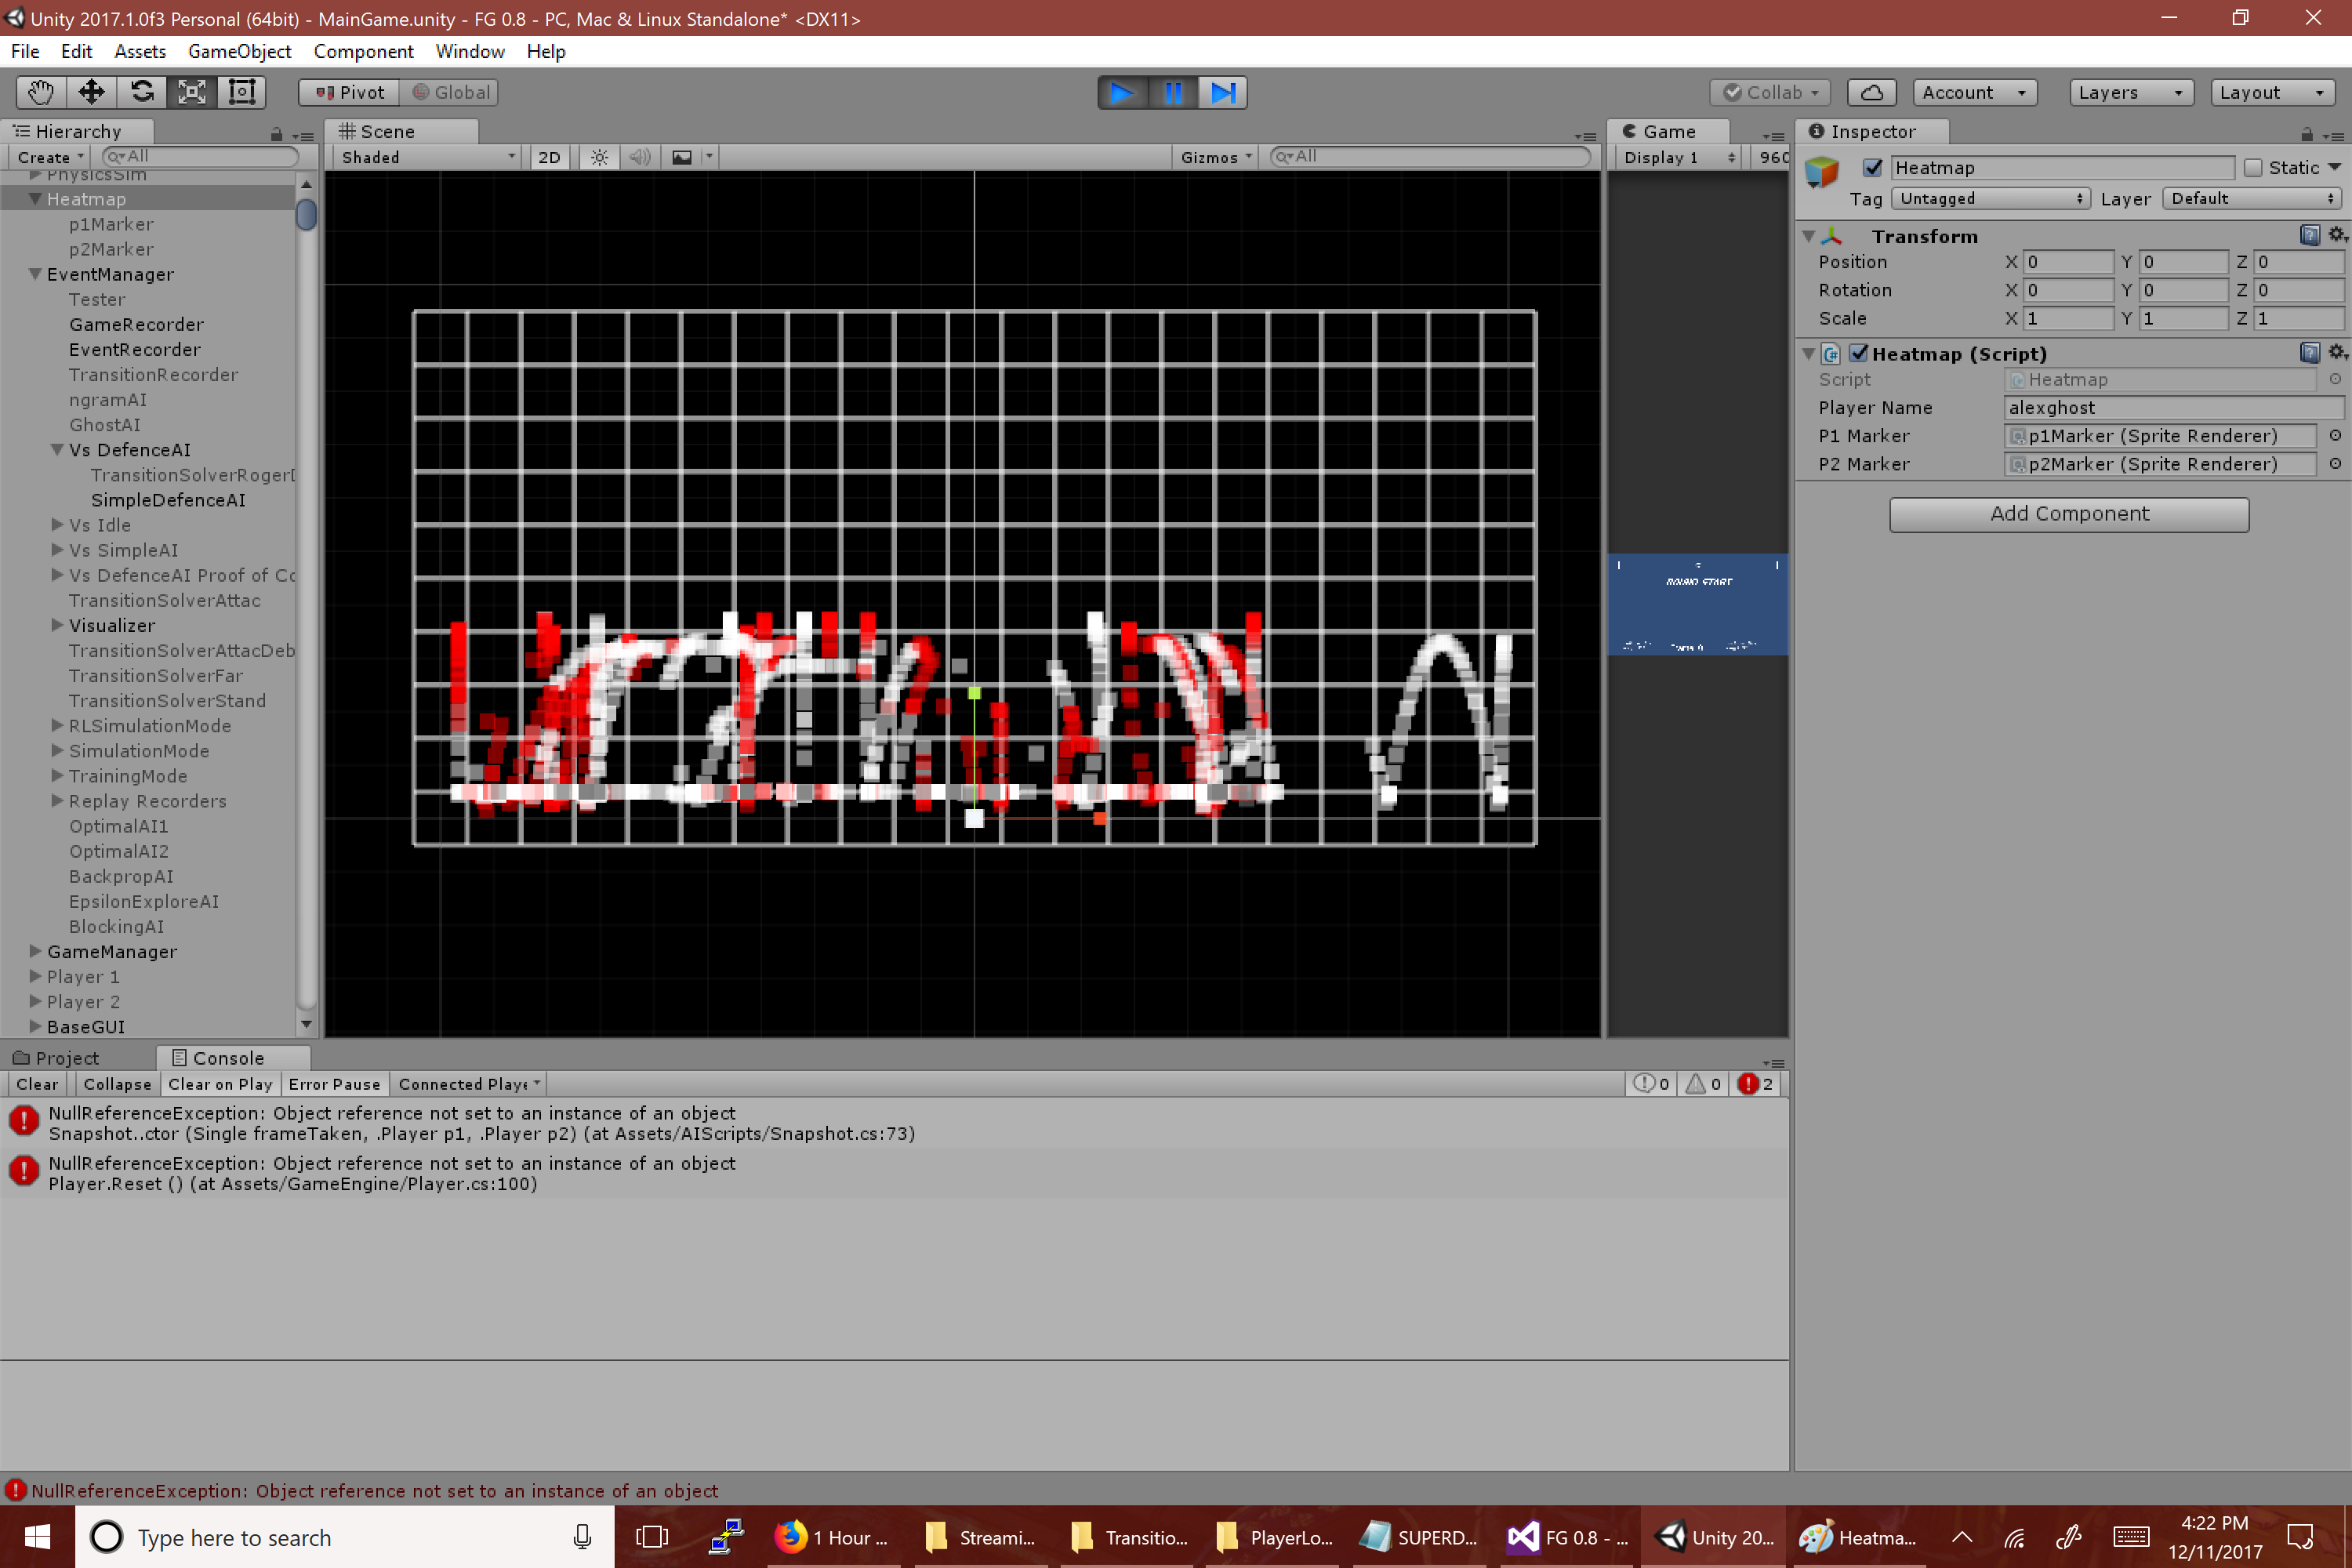
\includegraphics[width=\textwidth]{Figures/HeatmapGhost.png}
		\caption{GhostAI Heatmap}
		\label{}
	\end{subfigure}
	\begin{subfigure}[h]{0.4\textwidth}
		\centering
		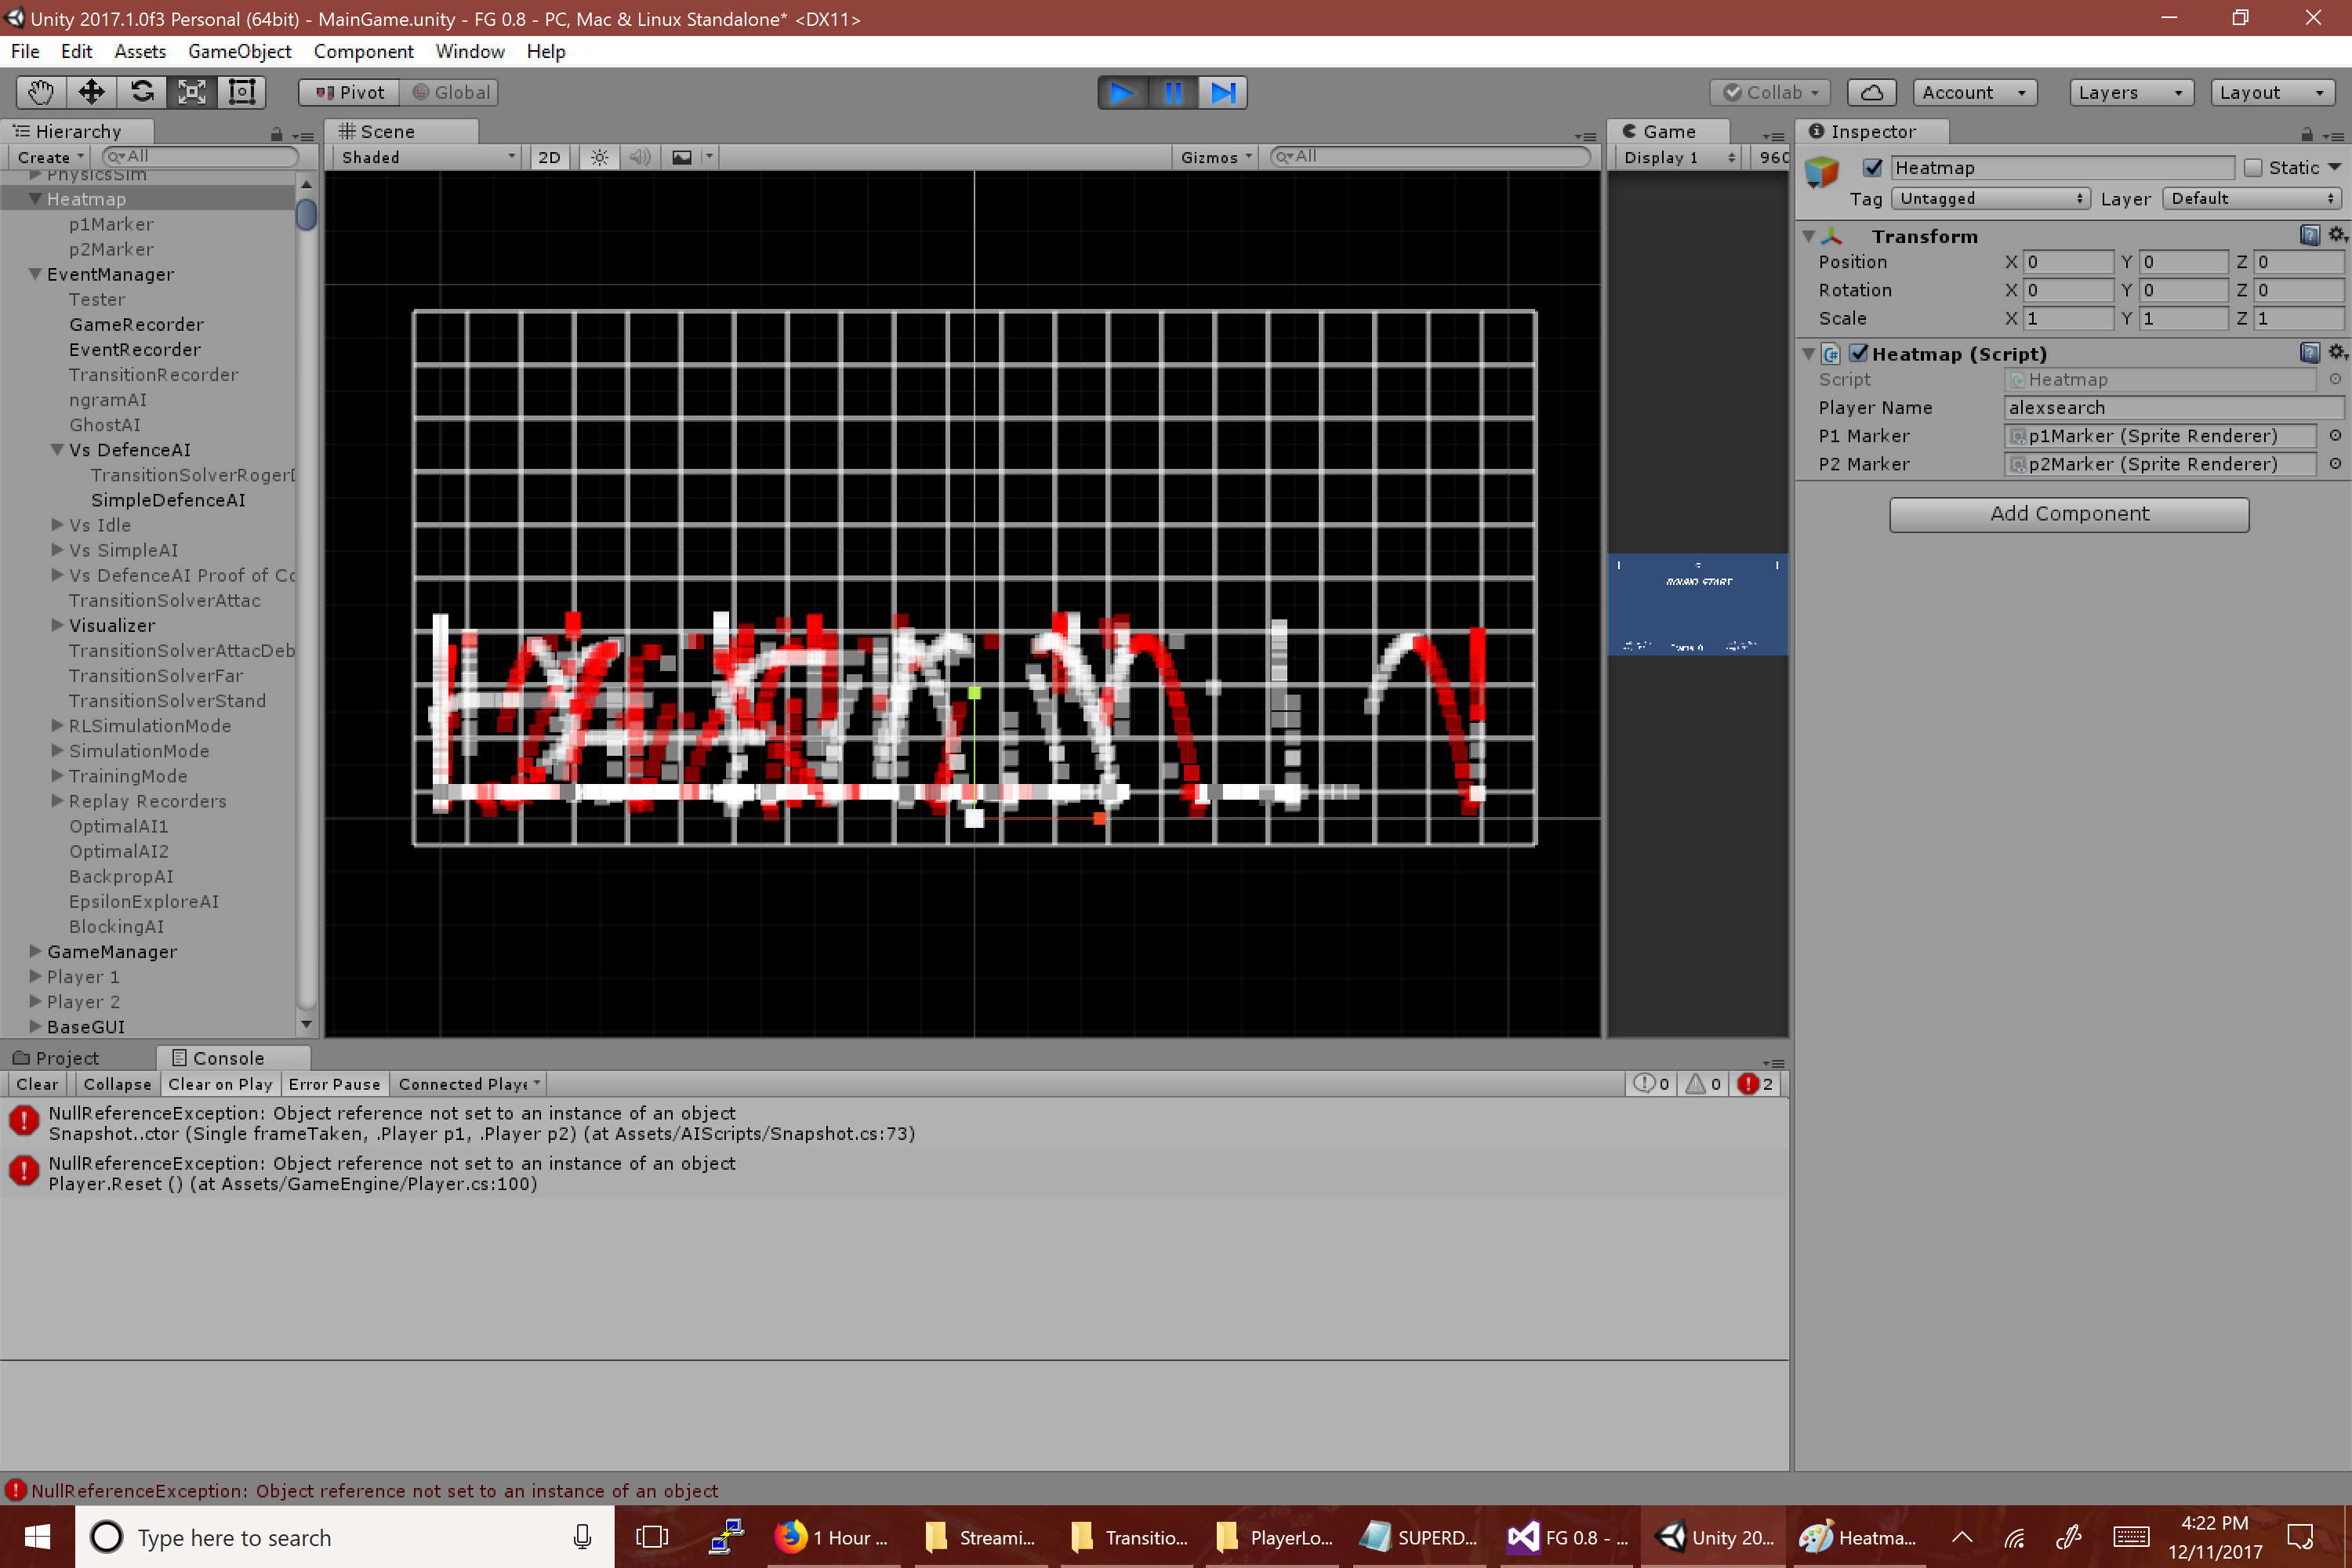
\includegraphics[width=\textwidth]{Figures/HeatmapAI.png}
		\caption{Search AI Heatmap}
		\label{}
	\end{subfigure}
\end{figure}

Lastly from a qualitative standpoint, it is hard to infer much from the heatmaps. They clearly show that Search AI and GhostAI are a step above the N-gram AI, but beyond that there is no clear delineation. Search AI seems to more accurately represent the grounded actions of the original player compared to GhostAI, but it is hard to tell the difference. However, in the video analysis, the Search AI's movement was the smoothest. This is because plannning allows it to take broad motions before deciding to take a different action. That said, both the Ghost AI and Search AI were prone to getting stuck into certain repeated patterns, a trait which to most people signifies a non-human player. This is likely because both GhostAI and Search AI try to reach the goal of hitting the opponent in an efficient manner. This adherence to an "optimal" kind of play can result in situations where the agent behaves greedily to a fault and comes off as non-human-like.


